% Junbiao Huang's mathematical control-journal report style.
\documentclass[lang=en,11pt,a4paper,bibend=bibtex]{elegantpaper}
\usepackage{xeCJK}
\setCJKmainfont{FandolSong-Regular.otf}
\setCJKsansfont{FandolSong-Regular.otf}
\setCJKmonofont{FandolSong-Regular.otf}
\usepackage{tikz,pgfplots,tabularx,titlesec,fancyhdr}
\usetikzlibrary{arrows.meta,positioning,calc}
\pgfplotsset{compat=1.18}
\geometry{left=23mm,right=23mm,top=21mm,bottom=22mm,headheight=15pt,headsep=7mm}
\linespread{1.10}
\setlength{\parindent}{0pt}
\setlength{\parskip}{5pt}
\setlength{\emergencystretch}{2em}
\definecolor{accent}{HTML}{234D64}
\definecolor{muted}{HTML}{59646C}
\definecolor{light}{HTML}{F0F4F6}
\hypersetup{colorlinks=true,linkcolor=accent,urlcolor=accent}
\titleformat{\section}{\Large\sffamily\bfseries\color{accent}}{\thesection}{0.6em}{}
\titleformat{\subsection}{\normalsize\sffamily\bfseries}{\thesubsection}{0.6em}{}
\titlespacing*{\section}{0pt}{9pt}{8pt}
\titlespacing*{\subsection}{0pt}{8pt}{3pt}
\pagestyle{fancy}
\fancyhf{}
\fancyhead[L]{\small\sffamily\color{muted}EXPERIMENT 2\enspace /\enspace ROBOMASTER EP}
\fancyhead[R]{\small\sffamily\color{muted}\studentname}
\fancyfoot[L]{\small\sffamily\color{muted}\studentid\quad\textbullet\quad Individual laboratory report}
\fancyfoot[R]{\small\sffamily\thepage}
\renewcommand{\headrulewidth}{0.3pt}
\renewcommand{\footrulewidth}{0pt}
\captionsetup{font=small,labelfont=bf,labelsep=period,skip=5pt,hypcap=false}
\renewcommand{\arraystretch}{1.18}
\newcolumntype{Y}{>{\raggedright\arraybackslash}X}
\newcommand{\code}[1]{{\small\nolinkurl{#1}}}
\newcommand{\source}[1]{{\small\color{muted}Source: #1}\par}
\newcommand{\reportnote}[1]{\par\smallskip\noindent\colorbox{light}{\parbox{\dimexpr\linewidth-2\fboxsep}{\small #1}}\par\smallskip}
\newcommand{\reporttitle}[1]{\vspace*{2mm}{\small\sffamily\bfseries\color{accent}FIXED-POINT PICK-AND-PLACE}\par\vspace{2mm}{\LARGE\sffamily\bfseries #1\par}\vspace{3mm}{\large\studentname\enspace\studentcn}\par{\small Student ID: \studentid\quad |\quad Individual report}\par\vspace{3mm}\hrule\vspace{3mm}}
\tikzset{box/.style={draw=accent,fill=light,rounded corners=2pt,align=center,font=\small,minimum height=9mm},arr/.style={-{Latex[length=2mm]},thick,draw=accent}}
\newcommand{\teamtable}{%
\par\smallskip
\begingroup\small\renewcommand{\arraystretch}{1.08}
\begin{tabularx}{\linewidth}{@{}>{\raggedright\arraybackslash}p{25mm}>{\raggedright\arraybackslash}p{21mm}Y@{}}\toprule
Member & Work area & Main responsibility \\\midrule
Ning Bo & Simulation & Set up the environment and scene; load models and launch the simulation.\\
Huang Junbiao & Simulation & Work on the motion program and debug grasping, transfer and repeated cycles.\\
Qi Yongyue & Simulation results & Organize logs, analyse results and prepare report material.\\
Bao Lintai & Hardware & SDK communication, task sequence, chassis turn/return and exception handling; joint trials.\\
Xue Yutong & Hardware & Pick/release waypoints, approach/lift heights, gripper adjustment and retention checks; joint trials.\\\bottomrule
\end{tabularx}\par\endgroup}
\newcommand{\commonrequirements}{%
\section{Experiment requirements and individual scope}
The experiment develops a fixed-point grasping task without visual localization: home, approach A, descend, grip, lift, transfer to B, release and return. The course requires a complete simulation launch, state publication, saved trajectories/results/errors, joint and reachability checks, and at least four successful transfers in five consecutive trials. Hardware verification additionally requires supervised low-speed operation, safe failure handling and individual safety-operation checks [1].

Because of equipment availability, our group used the DJI RoboMaster EP arm and gripper instead of the specified mechArm 270. The simulation uses ROS 2 Humble, Gazebo Fortress and custom kinematics/control on a Jetson Linux system. The physical implementation uses the RoboMaster Python SDK. This is a platform adaptation, not an unchanged ROS 2 hardware backend.
}
\newcommand{\commonlimits}{%
\reportnote{Scope of evidence. Simulation repeats A$\rightarrow$B and verifies home after every cycle; the object is reset only between cycles. Hardware alternates A/B, pauses for human grasp confirmation and returns home after all five cycles. Shared ROS 2 interfaces, parameter-only hardware switching and each member's safety check are not demonstrated by the supplied records.}}
\newcommand{\mainresults}{%
\begin{center}\small
\begin{tabular}{@{}crrrcc@{}}\toprule
Cycle & Error (mm) & Heading ($^\circ$) & Time (s) & Placed & Home \\\midrule
1 & 2.274 & 0.445 & 67.01 & Yes & Yes\\
2 & 5.604 & 0.329 & 59.72 & Yes & Yes\\
3 & 4.192 & 0.404 & 60.92 & Yes & Yes\\
4 & 4.577 & 0.459 & 61.09 & Yes & Yes\\
5 & 5.144 & 0.405 & 61.29 & Yes & Yes\\\bottomrule
\end{tabular}
\end{center}
\source{Recorded simulation run \code{20260913_153855_682865/results.json}; error is horizontal distance from configured B, heading is absolute home-heading error.}}
\newcommand{\hardwareresult}{%
\subsection{Physical validation: team-observed outcome}
The team confirmed that all five hardware transfers succeeded with no observed abnormalities. Cycles 1, 3 and 5 moved A$\rightarrow$B; cycles 2 and 4 moved B$\rightarrow$A. Each lift was followed by a fresh human \code{y} confirmation before rotation; final heading restoration and homing followed cycle 5. This is an observed 5/5 result, not an instrumented precision or timing measurement. No real-hardware position-error, duration or force data are available, and five successes do not establish long-run reliability.}
\newcommand{\githubsection}{%
\clearpage
\section{Shared GitHub repository and commit evidence}
The complete group archive is stored in the
\href{https://github.com/ccx8kg5qpd-debug/robomaster-ep-fixed-point-grasping}
{shared public GitHub repository}. The repository address is
\nolinkurl{github.com/ccx8kg5qpd-debug/robomaster-ep-fixed-point-grasping}.
It contains the simulation and hardware programs, model resources, saved results,
the complete simulation recording and all five individual report sources.

\begin{center}
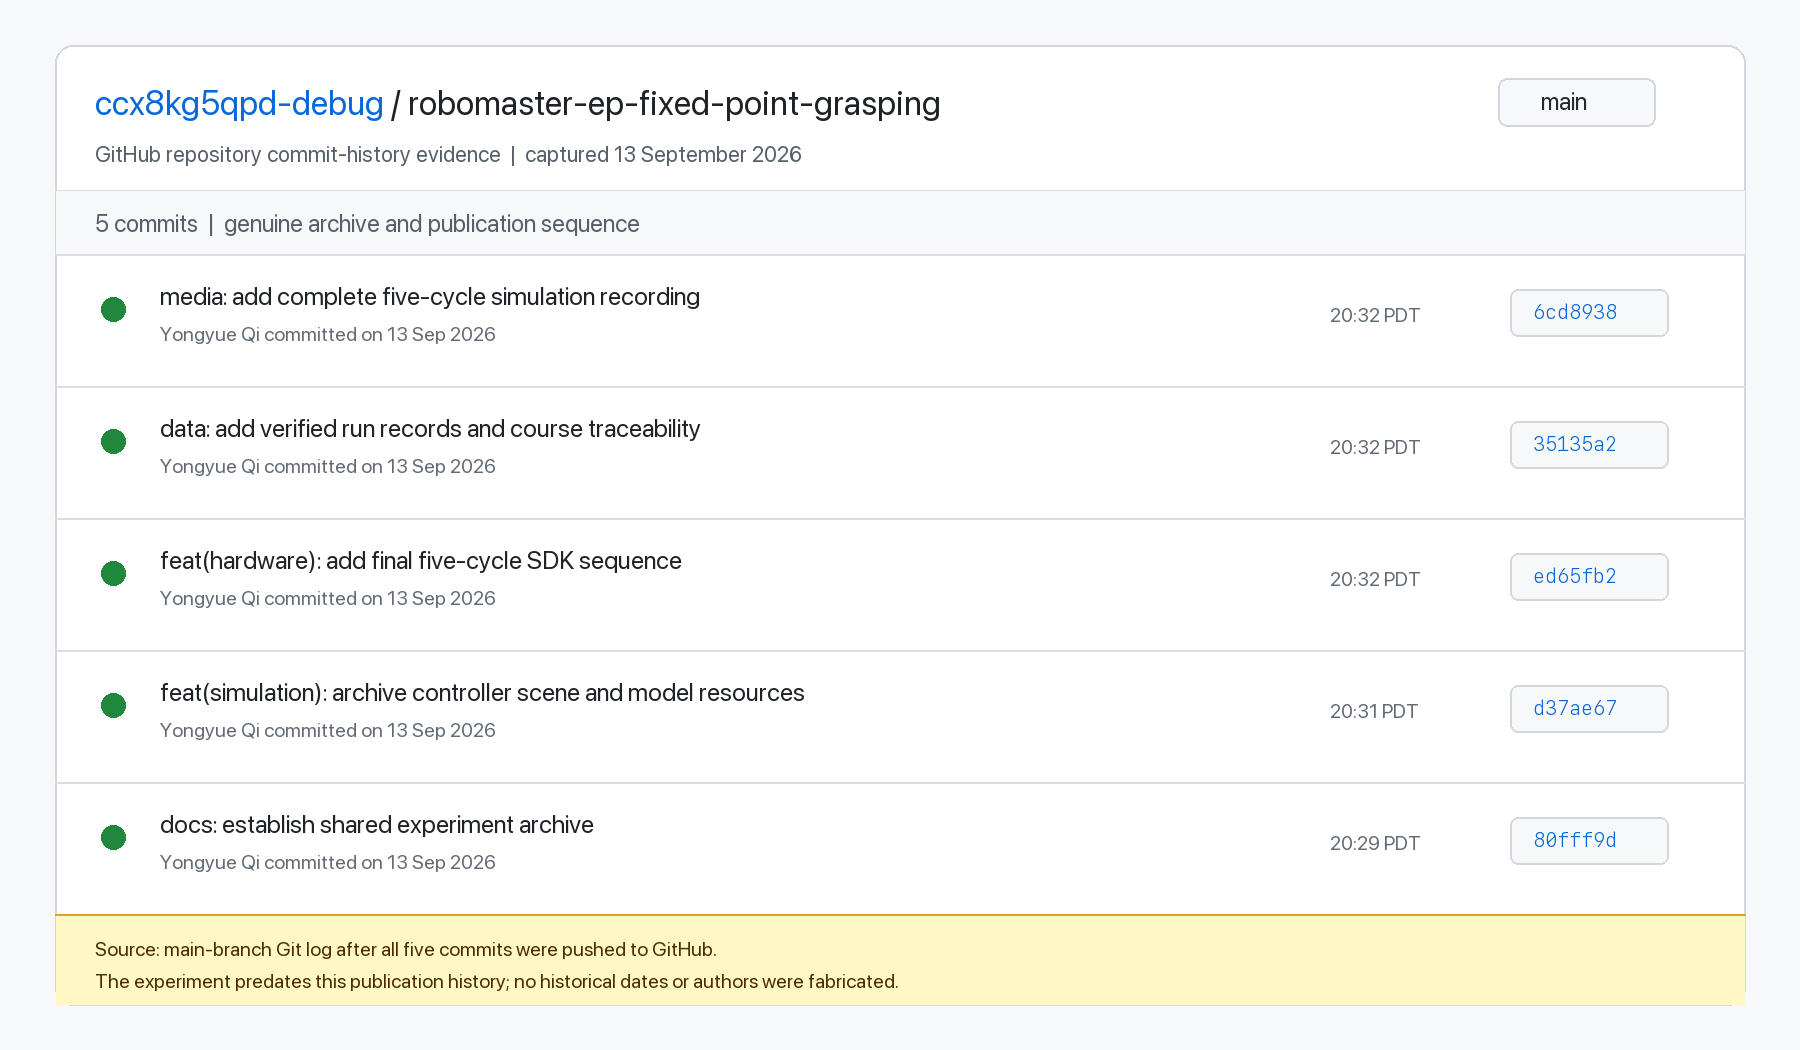
\includegraphics[width=\linewidth]{assets/commit_history_snapshot.png}
\captionof{figure}{Commit-history evidence captured after the first five project
materials commits had been pushed to the shared GitHub repository.}
\end{center}

\reportnote{Traceability note. The experiment was completed before the GitHub
repository was assembled. These genuine commits document the later review,
organization and publication sequence; they are not presented as a fabricated
contemporaneous development history. The screenshot records the five commits
visible at capture time, before this revised report was added.}
}
\newcommand{\referencesblock}{%
\section*{Sources and traceability}
{\footnotesize
[1] Course handout, \emph{Fixed-Point Robotic-Arm Grasping: Simulation Development and Hardware Validation}, S16--S20 / E5; individual-report assignment requirements.\par
[2] Shared team repository, \href{https://github.com/ccx8kg5qpd-debug/robomaster-ep-fixed-point-grasping}{robomaster-ep-fixed-point-grasping}, assembled 13 September 2026: simulation source/configuration, \code{real_v2_five_cycles_manual.py}, saved logs and reports. Primary numerical record: \code{20260913_153855_682865}.\par
[3] Team conversation fact-check materials, 13 September 2026, for development history; subsequent team confirmation for the completed five-cycle hardware run. Historical failures are not counted as final-run failures.\par
[4] Community model resources: \href{https://github.com/jeguzzi/robomaster_ros}{jeguzzi/robomaster\_ros}, archived commit \code{c05a39d7f0fa}. Report layout uses \href{https://ctan.org/pkg/elegantpaper}{ElegantPaper}, distributed under LPPL 1.3c.
}}

\definecolor{accent}{HTML}{7A2432}
\definecolor{muted}{HTML}{6E625E}
\definecolor{light}{HTML}{FBF4EC}
\definecolor{journalgold}{HTML}{B98737}
\geometry{left=25mm,right=25mm,top=22mm,bottom=23mm,headheight=16pt,headsep=7mm}
\hypersetup{linkcolor=accent,urlcolor=accent}
\titleformat{\section}{\Large\bfseries\color{accent}}{\Roman{section}.}{0.65em}{}
\titleformat{\subsection}{\normalsize\bfseries\itshape\color{accent}}{\thesubsection}{0.55em}{}
\fancyhead[L]{\small\scshape\color{muted}Motion Control Journal}
\fancyhead[R]{\small\color{muted}\studentname}
\fancyfoot[L]{\scriptsize\color{muted}Kinematics, sequencing and feedback logic}
\fancyfoot[R]{\small\bfseries\color{accent}\thepage}
\renewcommand{\headrulewidth}{0pt}
\renewcommand{\footrulewidth}{0.5pt}
\renewcommand{\reportnote}[1]{\par\smallskip\noindent\fcolorbox{journalgold}{light}{\parbox{\dimexpr\linewidth-2\fboxsep-2\fboxrule}{\small\textit{Control observation.} #1}}\par\smallskip}
\renewcommand{\reporttitle}[1]{\vspace*{5mm}{\small\scshape\color{journalgold}Robotics Integration Group Project I}\par\vspace{4mm}{\fontsize{23}{28}\selectfont\bfseries\color{accent}#1\par}\vspace{3mm}{\color{journalgold}\rule{32mm}{1.3pt}}\par\vspace{4mm}{\large\studentname\enspace\studentcn\par}{\small Student ID: \studentid\quad|\quad Individual control journal}\par\vspace{3mm}}

\newcommand{\studentname}{Huang Junbiao}
\newcommand{\studentcn}{黄俊彪}
\newcommand{\studentid}{24020036027}
\begin{document}
\reporttitle{Simulation Programming\\and Motion-Sequence Debugging}
\commonrequirements
\subsection{My responsibility and team interfaces}
My main responsibility is the simulation motion program and its debugging: moving through the waypoints, closing the gripper, coordinating the base turn and completing five cycles. Ning Bo prepares the environment and models, while Qi Yongyue organizes the resulting logs and analysis. Bao Lintai and Xue Yutong handle real-device operation. My report therefore explains both the motion calculations and how the controller decides when a simulated action is complete.
\teamtable
\commonlimits
\section{Kinematic model and reachability}
\subsection{Independent variables and coupled joints}
The RoboMaster EP mechanism should not be treated as a generic six-degree-of-freedom arm. The archived kinematic function uses two independent arm variables, $r$ and $l$, then derives linked joint coordinates. Examples include
\begin{equation}
q_{\mathrm{arm1}}=r,\quad q_{\mathrm{arm2}}=l-r,\quad
q_{\mathrm{endpoint}}=-l,\quad q_{\mathrm{rod}}=l.
\end{equation}
Gripper closure $g\in[0,1]$ is mapped to linked gripper coordinates by table interpolation. The simulation commands 21 arm/gripper/linkage joints; these are not 21 independent actuators. In particular, \code{gripper_m_joint} is prismatic and uses metres, whereas the rotational coordinates use radians.

Forward transforms are reconstructed from the SDF frame hierarchy. The two fingertip reference points lie near the forward ends of left and right gripper link 4. Their mean defines the grasp centre $\mathbf p_c$. The implemented inverse problem is
\begin{equation}
\min_{r,l}\left\|\begin{bmatrix}p_{c,x}(r,l,g)\\p_{c,z}(r,l,g)\end{bmatrix}
-\begin{bmatrix}x^*\\z^*\end{bmatrix}\right\|_2^2.
\end{equation}
SciPy least squares enforces $r\in[-0.274,1.384]$ and $l\in[-0.79936,1.73137]$. A further coupling check requires $r-l\in[-0.34732,1.21475]$. A residual norm above 0.002 m, or violation of the coupling condition, rejects the target instead of silently commanding an approximate pose.
\subsection{Waypoints and reference-frame discipline}
\begin{center}
\begin{tabular}{@{}lrrl@{}}\toprule
Waypoint & $x$ (m) & $z$ (m) & Purpose\\\midrule
Home & 0.235 & 0.220 & Retracted high configuration\\
Hover & 0.270 & 0.160 & Approach and transfer height\\
Grasp & 0.270 & 0.088 & Low fingertip-centre target\\\bottomrule
\end{tabular}
\end{center}
These are model tip-centre coordinates with a built-in 0.060 m vertical offset, not SDK coordinates and not object-centre heights. Operational opening uses $g=0.6$ rather than the table's fully open endpoint. The preflight checks home, hover and grasp with closure values 0.6 and 1.0. This checks selected endpoint solutions; it is not a complete swept-volume collision proof.
\clearpage
\section{Motion commands and the repeated sequence}
\subsection{A smooth reference between joint targets}
For a phase duration $T$, normalized time is $u=\mathrm{clip}((t-t_0)/T,0,1)$. The controller applies
\begin{equation}
s(u)=10u^3-15u^4+6u^5,\qquad
\mathbf q(t)=(1-s)\mathbf q_0+s\mathbf q_1.
\end{equation}
Both $s'$ and $s''$ vanish at the endpoints, reducing abrupt changes in the ideal commanded reference. This property does not guarantee zero measured acceleration in a contact simulation, and joint-space interpolation does not generally produce a straight Cartesian tip path.
\begin{center}
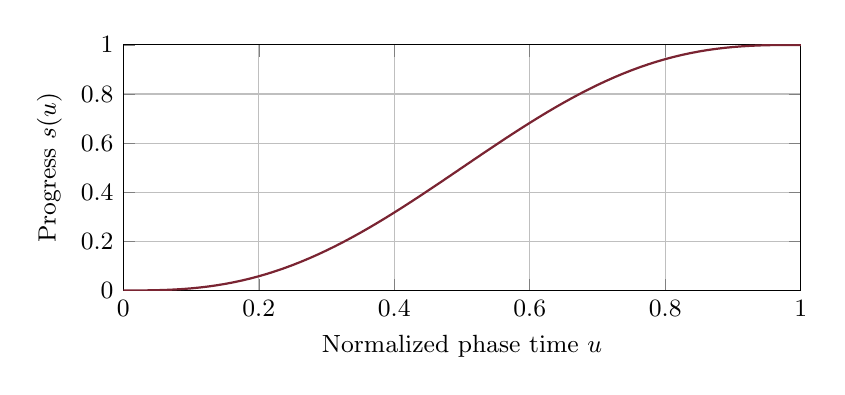
\begin{tikzpicture}
\begin{axis}[width=.84\linewidth,height=47mm,xmin=0,xmax=1,ymin=0,ymax=1,xlabel={Normalized phase time $u$},ylabel={Progress $s(u)$},grid=major,tick label style={font=\small},label style={font=\small}]
\addplot[accent,thick,domain=0:1,samples=81]{10*x^3-15*x^4+6*x^5};
\end{axis}
\end{tikzpicture}
\captionof{figure}{The analytical quintic reference used for joint interpolation; not measured telemetry.}
\end{center}
\subsection{Using the chassis to reach B}
The target points are $A=(0.278,-0.001,0.0725)$ m and $B=(0.237,0.1453,0.0725)$ m. During transfer, the desired heading is derived from the difference between the destination and grasped-object azimuths about the initial base position. Translation corrections are saturated at $\pm0.025$ m/s per commanded axis and yaw velocity at $\pm0.22$ rad/s. The simulation heading is therefore geometry-derived, not simply the hardware script's fixed $32^\circ$ command.

After release and retreat, the controller restores the original heading and then returns the arm home. The position/heading checks prevent a time-only sequence from assuming that a saturated base motion has already completed. This matters because the first recorded TURN phase lasts about 14.8 s despite a nominal 4 s phase reference.
\subsection{Connecting the actions into five cycles}
The ROS 2 node publishes joint targets and \code{/ep/cmd_vel}, and reads joint, pose and contact feedback. Its normal sequence is home, hover, descend, close, hold, lift, turn, lower, open and retreat, followed by placement checking, heading restoration and home verification. The final version records success only after the return is verified. Cycles 1--4 then enter \code{REFILL_WAIT}, allowing the separate refill node to reset the cube at A; cycle 5 ends at home. State messages and event records identify these transitions for debugging.
\clearpage
\section{Gripper feedback and experimental results}
\subsection{From contact detection to retained grasp}
During CLOSE, the controller requires contact entries from both gripper sides newer than 0.3 s, then sets $g_h=\min(1,g_{\mathrm{measured}}+0.04)$. HOLD has a nominal duration of 3 s. After that interval, recent bilateral contact and the arm/base completion conditions must remain satisfied for at least 0.4 s before lifting. It is not a fixed 3 s delay. The closure increment is a position preload, not a calibrated force command or weight measurement.

Successful lifting requires bilateral contact and object height above 0.135 m. A low object height during TURN can trigger a dropped-object failure. Lowering brings the object toward B; after opening and retreat, acceptance requires horizontal error below 23 mm, height error below 8 mm and table contact. Consequently, ``gripper closed'' alone is not sufficient evidence of a completed grasp.
\mainresults
The main simulation run completed all five transfers with home verification. The 4.358 mm mean horizontal placement error and 5.604 mm maximum are outcomes of the complete coupled system, not a direct measurement of IK residual. They include contact release, base positioning and settling effects. The 2 mm solver residual threshold applies to a different quantity: model fingertip target matching before execution.
\hardwareresult
\clearpage
\section{Problems, solutions and individual reflection}
\subsection{Selecting the correct grasp reference}
The kinematic source explicitly distinguishes the forward contact region of link 4 from the rear linkage at link 7. Using the wrong link could make an IK solution numerically excellent but physically irrelevant to the cube. The correct reference must represent where the fingertips actually hold the object, and its location must be checked against collision geometry.
\subsection{Unstable lifting and premature transfer}
The development record includes lift timeouts and grip instability. The final solution combines the 25 mm cube geometry, bilateral contact detection, a small closure preload and a holding interval before ascent. It would be unjustified to attribute all historical failures to one parameter: the notes describe several model and control changes. The defensible conclusion is that the final combination supports the recorded successful trials.
\subsection{A repeated grasp is not yet a complete repeated task}
An earlier revision lacked the requested return after every transfer. Explicit RETURN\_HEADING and RETURN\_HOME states resolve this problem; successful release alone no longer advances the cycle counter. The final main log has five placement checks, five home checks and four refill acknowledgments. This makes it possible to locate a failure by its phase instead of treating the whole experiment as one opaque loop.

The fact-check record reports four passing offline tests. The unreachable-target test calls the kinematic solver with $(x,z,g)=(10,10,0.6)$ and expects \code{ValueError}. This establishes solver-level rejection, not runtime stopping behavior. Stale-feedback and phase-timeout guards still need documented system-level fault tests. I would also sample the executed joint-space path for clearance, because valid IK endpoints do not prove that every intermediate configuration is safe.
\subsection{Main lesson and next improvement}
The project demonstrates that fixed points still require feedback: gripping, reaching and returning are different conditions. My main conclusion is to separate model solvability, smooth reference generation and physical task acceptance. A future unified task interface should expose those conditions explicitly for both Gazebo and the SDK backend, while retaining hardware-specific limits and a human confirmation checkpoint where automatic grasp sensing is insufficient.

No final-version system-level fault-injection results or measured hardware precision are supplied. The offline tests and nominal 5/5 outcome do not establish those separate properties.
\githubsection
\referencesblock
\end{document}
